% Section content template for individual Educative lessons
% This file contains the actual content for a specific section
% Generated from Educative API section content

% Section: Requirements of Google Docs’ Design
% Section ID: 5975395656007680
% Section Slug: requirements-of-google-docs-design
% Generated: 2025-12-08T15:22:46.831854

\subsection{Requirements}\label{xqks_xrwRYi0hYpxyZhv3}
\\
Let's look at the functional and non-functional requirements for designing a collaborative editing service.

\subsubsection{Functional requirements}\label{FSRVjcB-5F6tyekN3ABns}
\\
The activities a user will be able to perform using our collaborative document editing service are listed below:

\begin{itemize}
\item
\protect\phantomsection\label{yUg4xPANuvFmXZDN1KP7b}
\textbf{Document collaboration}: Multiple users should be able to edit a document simultaneously. Also, a large number of users should be able to view a document.
\item
\protect\phantomsection\label{d3fSuLo42OiSgmclGUqms}
\textbf{Conflict resolution}: The system should push the edits done by one user to all the other collaborators. The system should also resolve conflicts between users if they're editing the same portion of the document.
\item
\protect\phantomsection\label{LxJMo5R5Nyu16ne3dtRyU}
\textbf{Suggestions}: The user should get suggestions about completing frequently used words, phrases, and keywords in a document, as well as suggestions about fixing grammatical mistakes.
\item
\protect\phantomsection\label{uykosgcWlpwjF1yUY2CNu}
\textbf{View count}: Editors of the document should be able to see the view count of the document.
\item
\protect\phantomsection\label{M6jMnNplPVEMLAtt6tTto}
\textbf{History}: The user should be able to see the history of collaboration on the document.
\end{itemize}
\\
A real-world document editor also has to have functions like document creation, deletion, and managing user access. We focus on the core functionalities listed above, but we also discuss the possibility of other functionalities in the lessons ahead.

\begin{figure}[htbp]
 \centering
 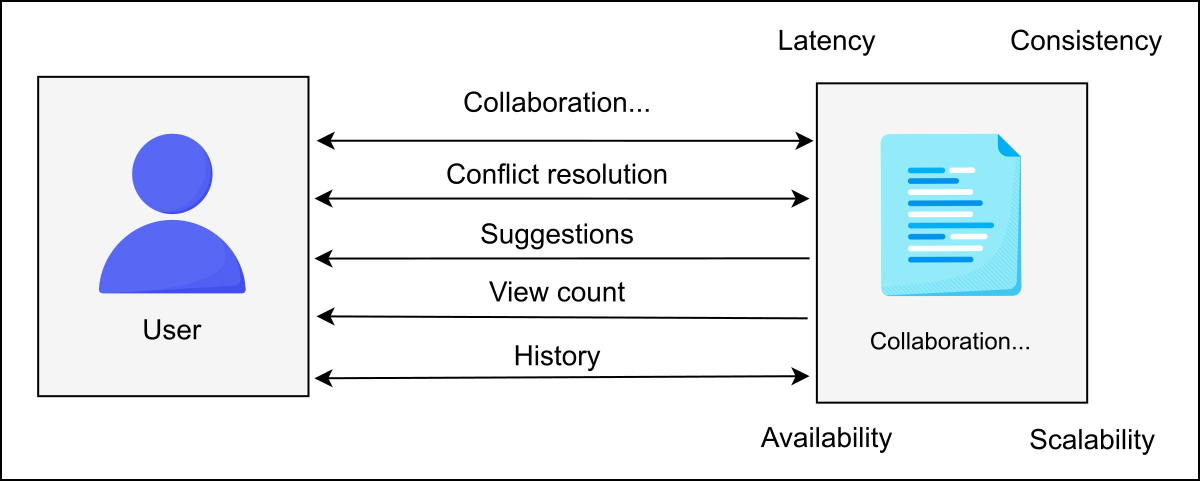
\includegraphics[width=0.5\textwidth]{Images/chapter_38/section_5975395656007680/5490981942460416.png}
 \caption{Functional and non-functional requirements of collaborative editing service}
\end{figure}

\subsubsection{Non-functional Requirements}\label{MHDDuopLlNkkfZ5g2DjkT}

\begin{itemize}
\item
\protect\phantomsection\label{0zpDeSieQRZg6iQ9MBph4}
\textbf{Latency}: Different users can be connected to collaborate on the same document. Maintaining low latency is challenging for users connected from different regions.
\item
\protect\phantomsection\label{aoN_ZVG3Ezw5Y0bGTChK_}
\textbf{Consistency}: The system should be able to resolve conflicts between users editing the document concurrently, thereby enabling a consistent view of the document. At the same time, users in different regions should see the updated state of the document. Maintaining consistency is important for users connected to both the same and different zones.
\item
\protect\phantomsection\label{A0lty6hnhxs0RRO7Ubvlc}
\textbf{Availability}: The service should be available at all times and show robustness against failures.
\item
\protect\phantomsection\label{tWpulkxeSfBfvlk63dtD_}
\textbf{Scalability}: A large number of users should be able to use the service at the same time. They can either view the same document or create new documents.
\end{itemize}

\subsection{Resource estimation}\label{7blonS_RyN0ah0vq7KJ4L}
\\
Let's make some resource estimations based on the following assumptions:

\begin{itemize}
\item
\protect\phantomsection\label{oneEqRn-2UdjuzTy1kL4G}
We assume that there are 80 million daily active users (DAU).
\item
\protect\phantomsection\label{xy6IS27y6wY48kZnDyH1m}
The maximum number of users able to edit a document concurrently is 20.
\item
\protect\phantomsection\label{WAI6ATX6Mk7nc_RVaf3sj}
The size of a textual document is 100 KB.
\item
\protect\phantomsection\label{vbOPtHuJMpDxbrOJ4a_sj}
30\% of all the documents contain images, whereas only 2\% of documents contain videos.
\item
\protect\phantomsection\label{vZSatrwhFtJffeaQkwBYr}
The collective storage required by images in a document is 800 KB, whereas each video is 3 MB.
\item
\protect\phantomsection\label{w0htPh2QmhXDFSEI42PVF}
A user creates one document in one day.
\end{itemize}
\\
Based on these assumptions, we'll make the following estimations.

\subsubsection{Storage estimation}\label{s-RrBRrFdhBXWFz-2modg}
\\
Considering that each user is able to create one document a day, there are a total of 80 million documents created each day. Below , we estimate the storage required for one day:
\begin{quote}
\textbf{Note:} We can adjust the values in the table below to see how the storage requirement estimations change.
\end{quote}

\begin{itemize}
\tightlist
\item
Total number of documents in a day: \(80M \times 1 document = 80M\) documents in a day
\item
Storage for each textual document: \(80M \times 100KBs = 8 TBs\)
\item
Storage required for images for one day: \(\frac{80M \times 30}{100} \times 800KBs = 19.2 \ TBs\) (Thirty percent of documents contain images.)
\item
Storage required for video content for one day: \(\frac{80M \times 2}{100} \times 3 MBs = 4.8 \ TBs\) (Two percent of documents contain videos.)
\end{itemize}

\begin{figure}[htbp]
 \centering
 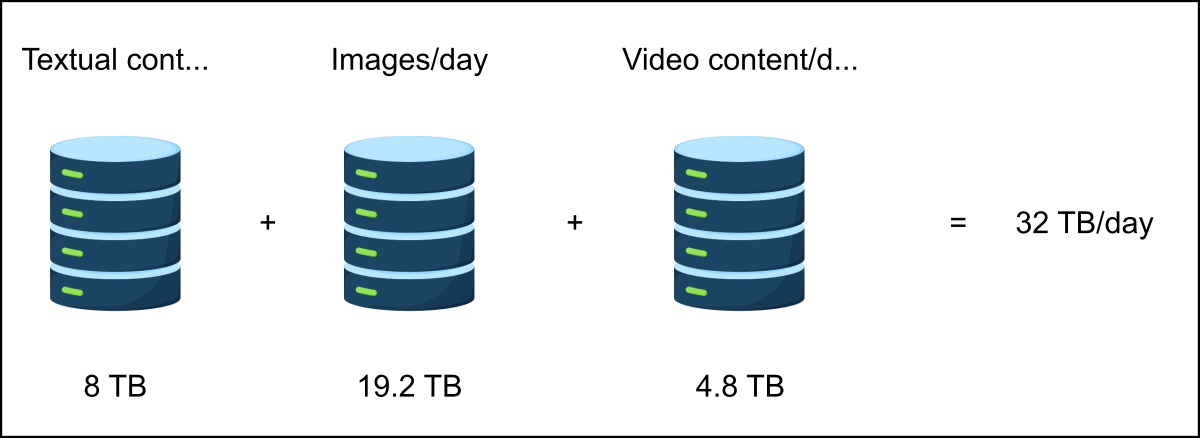
\includegraphics[width=0.5\textwidth]{Images/chapter_38/section_5975395656007680/4798384475340800.png}
 \caption{Storage required by online collaborative document editing service per day}
\end{figure}

Total storage required for one day is as follows: \protect\phantomsection\label{katex_inline_MFHM-SGHocTTswdu25nrD}{{{\(8 + 19.2 + 4.8 = 32\ \text{TBs}\)}}} per day
\begin{quote}
\textbf{Note:} Although our functional requirements state that we should keep a history of documents, we didn't include storage requirements for historical data for the sake of brevity.
\end{quote}
\subsubsection{Bandwidth estimation}\label{JN1wRvj0VT94CDf_8D1he}
\\
\textbf{Incoming traffic}: Assuming that 32 TB of data are uploaded per day to the network of a collaborative editing service, the network requirement for incoming traffic will be the following:
\\
\protect\phantomsection\label{katex_inline_q-eccZS3A0P2gWtZ2jMLI}{{{\(\frac{32\ \text{TB}}{86400} \times 8 = 3 \text{Gbps}\)}}} approximately
\\
\textbf{Outgoing traffic}: To estimate outgoing traffic bandwidth, we'll assume the number of documents viewed by a user each day. Let's consider that a typical user views five documents per day. Then, the following calculations apply:
\begin{quote}
\textbf{Note:} We can adjust the values in the table below to see how the calculations change.
\end{quote}

\begin{itemize}
\tightlist
\item
Total documents viewed per day by all users: \(80 M \times 5 = 400 M\) documents viewed per day
\item
Documents viewed per second: \(\frac{400 M}{86400} = 4.6 \times 10^3\) documents viewed per second
\item
Calculating the bandwidth required for textual content: \(4.6 \times 10^3 \times 100 KB \times 8 = 3.7 Gbps\)
\item
Calculating the bandwidth required for image-based content: \(\frac{4.6 \times 10^3 \times 30}{100} \times 800 KB \times 8 = 8.8 Gbps\)
\item
Calculating the bandwidth required for video content: \(\frac{4.6 \times 10^3 \times 2}{100} \times 3 MB \times 8 = 2.2 Gbps\)
\item
Total outgoing bandwidth: \(3.7 + 8.8 + 2.2 = 14.7 Gbps\)
\end{itemize}

\begin{figure}[htbp]
 \centering
 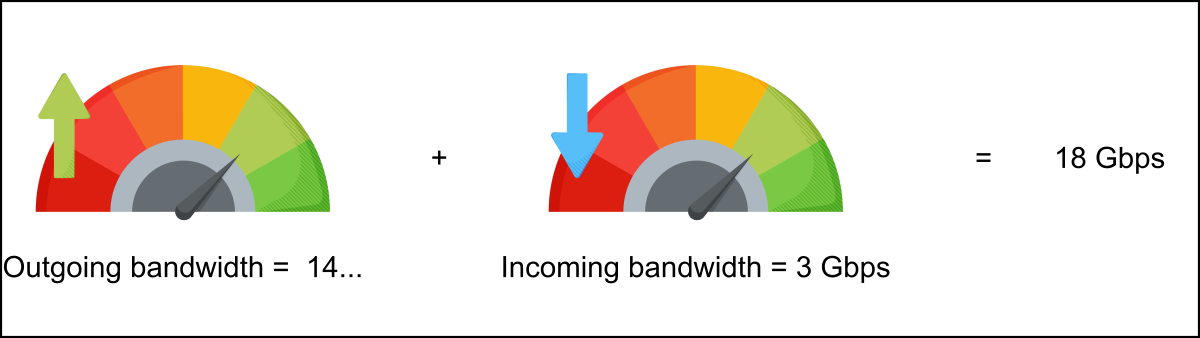
\includegraphics[width=0.5\textwidth]{Images/chapter_38/section_5975395656007680/6065391288057856.png}
 \caption{The total bandwidth required by Google Docs}
\end{figure}

\begin{quote}
\textbf{Note:} The total bandwidth required is equal to the sum of incoming and outgoing traffic. \protect\phantomsection\label{katex_inline_gN8r_Kpsgz85acQnoayuB}{{{\(= 3+14.7≈18\text{Gbps}\)}}} approximately.
\end{quote}
\subsubsection{Number of servers estimation}\label{Txv54Aro_9FoQCFVeqCOE}
\\
Since we have 80 million daily active users working on collaborative documents. Considering
\href{https://www.educative.io/courses/grokking-the-system-design-interview/put-back-of-the-envelope-numbers-in-perspective}{our assumption} of using daily active users as a proxy for the number of requests per second to find the number of servers for peak load times, we get 80 million requests per second. Then
, we use the following formula to calculate the number of servers:

\[
\text{Servers needed at peak load} = \frac{\text{Number of requests/second}}{\text{RPS of server}}
\]

Using \href{https://www.educative.io/courses/grokking-the-system-design-interview/put-back-of-the-envelope-numbers-in-perspective}{64,000 as an estimated RPS a server can handle}, the required servers are estimated as follows:

\[
\text{Servers needed at peak load} = \frac{80\ \text{million}}{64,000} = 1250 \approx 1.3\ \text{K servers}
\]

\begin{figure}[htbp]
 \centering
 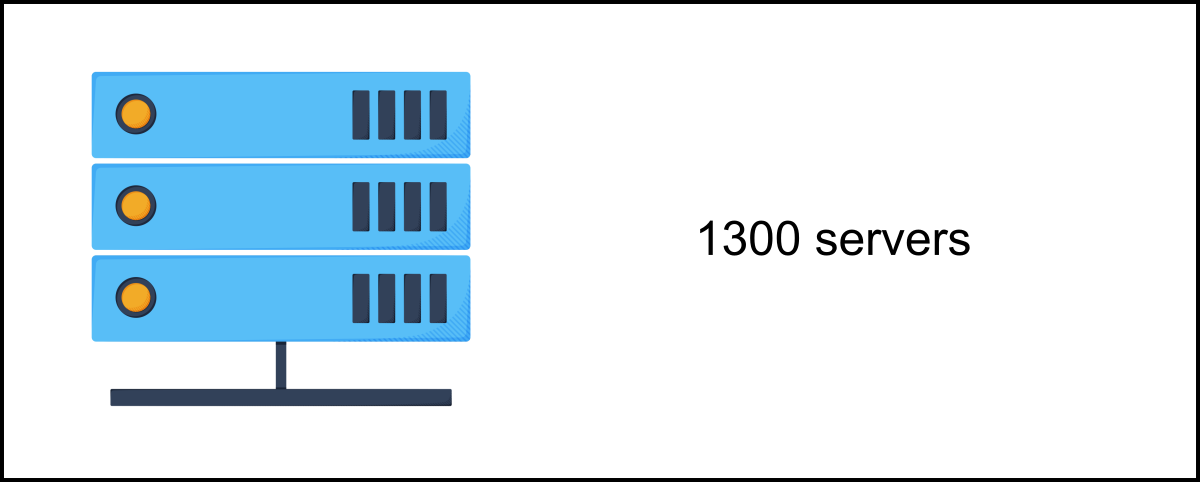
\includegraphics[width=0.15\textwidth]{Images/chapter_38/section_5975395656007680/5311998978293760.png}
 \caption{The estimated number of servers required for Google Docs}
\end{figure}

\subsection{Building blocks we will use}\label{YCxihRdU6S3SjrNSnEbXI}
\\
We'll use the following building blocks in designing the collaborative document editing service.

\begin{figure}[htbp]
 \centering
 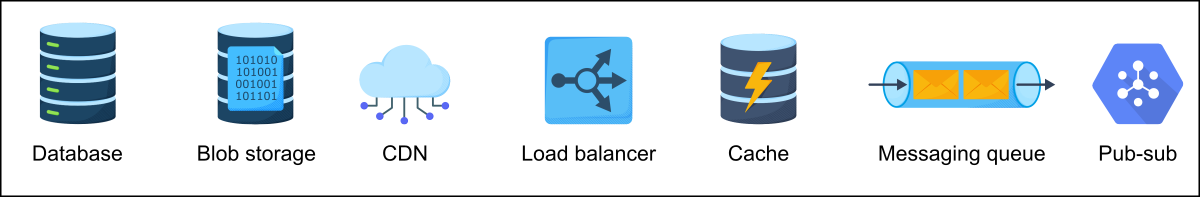
\includegraphics[width=0.5\textwidth]{Images/chapter_38/section_5975395656007680/4846865713856512.png}
 \caption{Building blocks required to be integrated in the design}
\end{figure}

\begin{itemize}
\item
\protect\phantomsection\label{fEWLlqO04qkwFECZpqH1l}
\href{https://www.educative.io/courses/grokking-the-system-design-interview/introduction-to-databases}{\textbf{Databases}} will be needed to store several things including textual content, history of documents, user data, etc. For this purpose, we may need different types of databases.
\item
\protect\phantomsection\label{hdiVsBxEYV-4s08zbcb_f}
\href{https://www.educative.io/courses/grokking-the-system-design-interview/system-design-a-blob-store}{\textbf{Blob storage}} will store large files, such as images and videos.
\item
\protect\phantomsection\label{AYt7_1WZMuYb_3F_O1dnE}
\href{https://www.educative.io/courses/grokking-the-system-design-interview/system-design-the-content-delivery-network-cdn}{\textbf{A CDN}} can store frequently accessed media in a document. We can also put read-only documents that are frequently requested in a CDN.
\item
\protect\phantomsection\label{TvZPn_keI7gx6965e6K28}
\href{https://www.educative.io/courses/grokking-the-system-design-interview/introduction-to-load-balancers}{\textbf{Load balancers}} will be the first point of contact for users.
\item
\protect\phantomsection\label{f6wXd0Sw2peKjDXwKgUZh}
\href{https://www.educative.io/courses/grokking-the-system-design-interview/system-design-the-distributed-cache}{\textbf{Caching}} will help us improve the performance of our design.
\item
\protect\phantomsection\label{FfIQ2Rn2yAnswp0vo-hZu}
\href{https://www.educative.io/courses/grokking-the-system-design-interview/system-design-the-distributed-messaging-queue}{\textbf{A Queueing system}} will queue editing operations requested by different users. Because many editing requests can't be performed simultaneously, we have to temporarily put them in a queue.
\item
\protect\phantomsection\label{oIakc5nuRg3cqRJZw-qoU}
\href{https://www.educative.io/courses/grokking-the-system-design-interview/system-design-the-pub-sub-abstraction}{\textbf{Pub-sub}} systems can complete tasks that can\textquotesingle t be performed right away. We\textquotesingle ll complete a number of tasks asynchronously in our design. Therefore, we\textquotesingle ll use a pub-sub system.
\end{itemize}

% End of section content